\begin{figure}[h]
\centering
\newcommand{\myWidth}{0.28\textwidth}
\newcommand{\myspace}{\hspace{3mm}}
\begin{subfigure}{\myWidth}
  \centering
  \caption{Probability of Success (Tanh, Scaled Gaussian Init.)}
  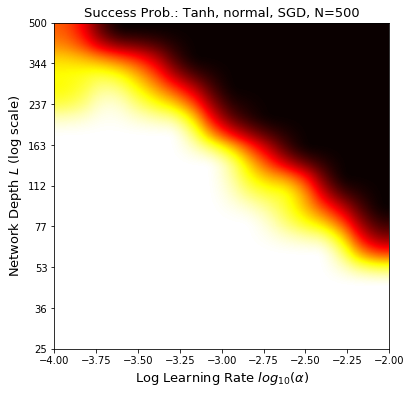
\includegraphics[width=1.0\linewidth,trim={0 0 0 0.65cm},clip]{s_tanh_normal_sgd}
  \label{fig:mnist_sgd_s1}
\end{subfigure}\myspace%
\begin{subfigure}{\myWidth}
  \centering
  \caption{Probability of Success (ReLU, Scaled Gaussian Init.)}
  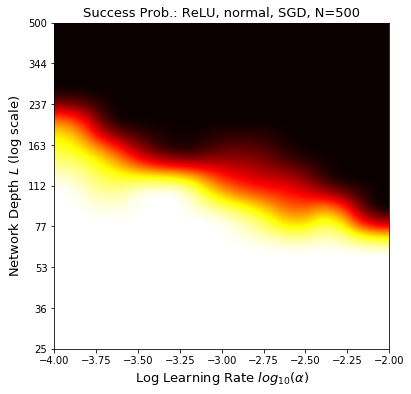
\includegraphics[width=1.0\linewidth,trim={0 0 0 0.65cm},clip]{s_relu_normal_sgd}
  \label{fig:mnist_sgd_s2}
\end{subfigure}\myspace
\begin{subfigure}{8mm}
  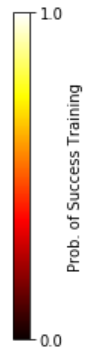
\includegraphics[width=\linewidth]{s_colorbar}
\end{subfigure}%
\\
\begin{subfigure}{\myWidth}
  \centering
  \caption{Probability of Success (Tanh, Orthogonal Init.)}
  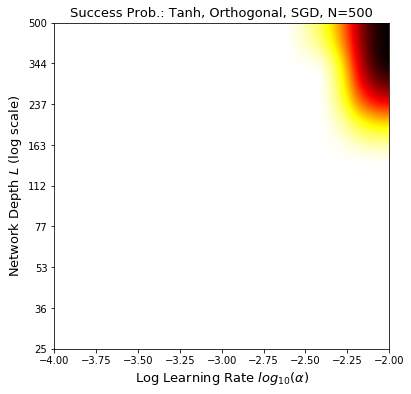
\includegraphics[width=1.0\linewidth,trim={0 0 0 0.65cm},clip]{s_tanh_orthogonal_sgd}
  \label{fig:mnist_sgd_s3}
\end{subfigure}\myspace
\begin{subfigure}{\myWidth}
  \centering
  \caption{Probability of Success (ReLU, Orthogonal Init.)}
  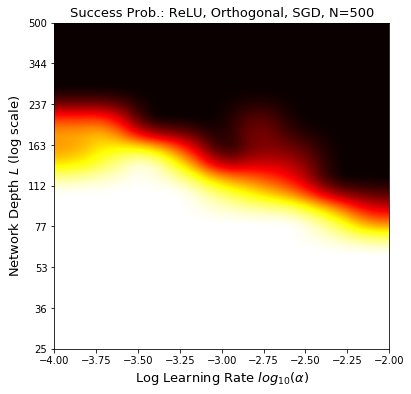
\includegraphics[width=1.0\linewidth,trim={0 0 0 0.65cm},clip]{s_relu_orthogonal_sgd}
  \label{fig:mnist_sgd_s4}
\end{subfigure}\myspace
\begin{subfigure}{8mm}
  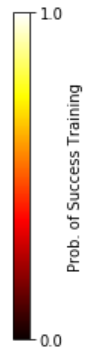
\includegraphics[width=\linewidth]{s_colorbar}
\end{subfigure}%
  % \caption{Final $R_{sq}$ (Tanh, Scaled Gaussian Init.), the initial $R_{sq}=0.304\pm0.210$.}
  % \caption{Final $R_{sq}$ (Tanh, Orthogonal Init.), the initial $R_{sq}=0.031\pm0.000$.}
  % \caption{Final $R_{sq}$ (ReLU, Orthogonal Init.), the initial $R_{sq}=0.788\pm0.239$.}
% Initial $0.304\pm0.210$, $0.031\pm0.000$ and $1$,
% the final VNI $R_{sq}$ of success/failure are $0.299\pm0.091/0.980\pm0.056$, $0.234\pm0.060/0.945\pm0.133$ and $0.424\pm0.199/0.944\pm0.118$ respectively. 
\caption{Probability of successful training for different network depth $L$ and learning rate $\alpha$ (the SGD optimizer). The networks are initialized with scaled Gaussian/orthogonal weights with Tanh/ReLu activation functions.
%We observe that the difficulty of training arises when the VNI $R_{sq}$ increases to 1.
%, and that the orthogonal weight initialization can reduce the probability of failure.
}
\label{fig:mnist_sgd}
\end{figure}